%ACM journals format:
\documentclass[prodmode,acmtodaes]{acmsmall} 
\usepackage[ruled]{algorithm2e}
\usepackage{multirow}
\renewcommand{\algorithmcfname}{ALGORITHM}
\SetAlFnt{\small}
\SetAlCapFnt{\small}
\SetAlCapNameFnt{\small}
\SetAlCapHSkip{0pt}
\IncMargin{-\parindent}

%Springer DAES format below:
%\documentclass[runningheads,a4paper]{llncs}
%\usepackage{amssymb}
%\setcounter{tocdepth}{3}
%\usepackage{graphicx}

% Metadata Information
%\acmVolume{9}
%\acmNumber{4}
%\acmArticle{39}
%\acmYear{2010}
%\acmMonth{3}

% Document starts
\begin{document}

% Page heads
\markboth{I. Filippopoulos et al.}{Data Interleaving and Memory Mapping on SIMD architectures}

% Title portion
\title{Integrated Exploration Methodology for Data Interleaving and Data-to-Memory Mapping on SIMD architectures}
\author{IASON FILIPPOPOULOS
\affil{Norwegian University of Science and Technology}
NAMITA SHARMA 
\affil{Indian Institute of Technology Delhi}
FRANCKY CATTHOOR
\affil{IMEC \& K.U. Leuven}
PER GUNNAR KJELDSBERG
\affil{Norwegian University of Science and Technology}
PREETI PANDA
\affil{Indian Institute of Technology Delhi}
}

\begin{abstract}
This work presents a methodology for efficient exploration of data interleaving and data-to-memory mapping options for SIMD (Single Instruction Multiple Data) platform architectures.
The system architecture consists of  a reconfigurable clustered scratch-pad memory and a SIMD function unit, which performs the same operation on multiple input data in parallel. 
The memory accesses have an important contribution on the overall energy consumption of an embedded system executing a data intensive task. 
The scope of this work is the reduction of the overall energy consumption by increasing the utilization of the function units and decreasing the number of memory accesses.
The presented methodology is tested using a number of benchmark applications with irregularities on their access scheme.
Potential gains are calculated based on the energy models both for the processing and the memory part of the system.
The improvement on the energy consumption after efficient interleaving and mapping of data is approximately between 40\% and 80\% for the complete system and the studied benchmarks.
\end{abstract}

\category{D.2.2}{Design Tools and Techniques}{Design, Methodologies}
\category{B.7.1}{Types and Design Styles}{Memory Technologies, Design}
\category{B.8.2}{Performance Analysis and Design Aids}{}
\category{C.3}{Special purpose and Application-Based Systems}{Real-time and Embedded Systems}
\category{E.1}{Data Structures}{Arrays}

\terms{Design, Algorithms, Performance}

\keywords{Data Interleaving, Single Instruction Multiple Data (SIMD) Architectures, Design Space Exploration, Memory Reconfiguration, Data Layout, Energy Optimization}

\acmformat{Iason Filippopoulos, Namita Sharma, Francky Catthoor, Per Gunnar Kjeldsberg, Preeti Panda, 2015. Integrated Optimization Methodology for Data Interleaving and Memory Mapping Exploration on SIMD architectures.}

\begin{bottomstuff}
Author's addresses: Iason Filippopoulos {and} Per Gunnar Kjeldsberg, Department of Electronics and Telecommunications, Norwegian University of Science and Technology (NTNU), Hogskoleringen 1, 7491 Trondheim, Norway; Namita Sharma  {and} Preeti Panda, Department of Computer Science and Engineering, Indian Institute of Technology Delhi, Hauz Khas, New Delhi - 110016, India; Francky Catthoor, Interuniversity Microelectronics Centre and K. U. Leuven, Kapeldreef 75, B-3001 Leuven, Belgium.
\end{bottomstuff}



\maketitle

\section{Introduction}

The energy is an important limitation factor on modern embedded systems.
New novel hardware solutions have been proposed to reduce the energy consumption.
On the processing side, SIMD architectures offer new possibilities for potential improvements on the performance and the energy consumption.
On the memory side, modern memory architectures provide different energy modes and clustered scratch-pad memory banks can operate independently offering more options for reducing energy consumption.
Dynamic and data intensive algorithms are implemented on embedded systems.
Data intensive applications have often irregular memory accesses, meaning that the data in memory are not accessed always in order.
The lack of spatial locality and the presence of redundant data results in lower utilization of the hardware resources, providing that a conventional approach is employed for the handling of data.
This problem motivates the development of a methodology to improve the management of the data.

In order to tackle this problem we propose an interleaving exploration that aims to increase spatial locality and reduce the memory accesses on redundant data.
The goal of this work is to improve the energy consumption for data intensive applications without any loss on the application's performance. 
We focus on single instruction multiple data (SIMD) architectures and explore applications that have irregularities on their access scheme. 
SIMD architectures can potentially increase the performance of an application, providing that the utilization of them is high. 
However, applications with irregular access patterns do not provide compact sequences of data that are suitable for high utilization. 
Hence the performance is lower than expected and the number of memory accesses is high due to redundant memory accesses. 
In order to reduce the number of memory accesses and achieve higher utilization of the system architecture a systematic exploration of the interleaving options for application's data is needed. 

The energy consumption can be divided into two parts, namely the processing and the memory subsystem. 
The energy needed for processing depends mainly on the utilization of the FUs and any potential stalls, if the memory cannot provide data on the needed rate.
The interleaving exploration can increase the utilization of the processing subsystem and reduce time penalties for data loading.   
The energy consumption on the memory subsystem is affected by the number of memory accesses and the energy per access. 
Again, the memory architecture and the data-to-memory mapping decisions have a great impact on both the number of accesses and the energy per access.

This article is organized as follows. 
Section~\ref{sec:motivational} motivates the study of developing a methodology for optimization of the data interleaving exploration and the data-to-memory mapping. 
Section~\ref{sec:related} surveys related work on both the interleaving and memory mapping exploration.
Section~\ref{sec:methodology} presents the general work-flow and the sequence of the methodology steps.
In Section~\ref{sec:platform} the target platform is described accompanied by a detailed description of the employed SIMD architecture and the memory models, while the set of benchmarks and their characteristics are analysed in Section~\ref{sec:applications}. 
Results of applying the described exploration methodology to the targeted applications are shown in Section~\ref{sec:results}, while conclusions are drawn in Section~\ref{sec:conclusion}. 

A large number of papers have demonstrated the importance of the memory organization to the overall system energy consumption. 
As shown in \cite{Gonzalez1996} memory contributes around 40\% to the overall power consumption in general purpose systems. 
Especially for embedded systems, the memory subsystem accounts for up to 50\% of the overall energy consumption \cite{Che09} and the cycle-accurate simulator presented in \cite{Ben99} estimates that the energy expenditures in the memory subsystem range from 35\% up to 65\% for different architectures. 
The breakdown of power consumption for a recently implemented embedded system presented in \cite{Hul11} shows that the memory subsystem consumes more than 40\% of the leakage power on the platform. 
According to \cite{tcm}, conventional allocation and assignment of data done by regular compilers is suboptimal. 
Performance loss is caused by stalls for fetching data and data conflicts for different tasks, due to the limited size of memory and the competition between tasks. 

\section{Motivational Example}
\label{sec:motivational}

To illustrate the sub-optimal utilization of SIMD architectures using conventional allocation and assignment of data, the simple example of Alg.~\ref{alg:motivation} is used.
In this example, we assume that the desired result is always the sum of 4 elements from arrays \textit{A, B, C and D}. 
The access pattern shows an irregularity, as a result of the iteration index.
For every group of four sequential array elements, there is only one used for the calculation of the result and the other three are skipped.
An intuitive interleaving optimization is the interleaving of the arrays \textit{A, B, C and D}, in order to generate sequences of elements that are all useful on the calculation of the \textit{result} variable. 
A full interleaving exploration could reveal several options to produce larger sequences of array elements that are needed during the execution of Alg.~\ref{alg:motivation}.
For example, the interleaving of every fourth line within the combined array ($A\vert B\vert C\vert D$) result in a sequence of 8 accessed elements.

\begin{algorithm}[t]
\SetAlgoNoLine
$N \leftarrow 100$ \newline
\For{($i = 0; i < N; i+4$)}{
        ${result(i) = A(i) + B(i) + C(i) + D(i)}$\;
}
\caption{Motivational Example Algorithm}
\label{alg:motivation}
\end{algorithm}

The initial data representation for the arrays \textit{A, B, C and D} is shown in Fig.\ref{fig:motivation}(a). 
The array elements that are accessed during the execution of the motivational example are marked with colors, in contrast to the elements that are not accessed.
The array elements are drawn in 25 lines with 4 elements on each line only for a better visual representation.
At this point there is no mapping to the memory architecture and no constrain regarding the number of lines or their width on the memory design.
The interleaving of the arrays \textit{A, B, C and D} is shown in Fig.\ref{fig:motivation}(c). 
Each line of the new interleaved array contains one elements from the initials arrays.
For example, the first line consists of the elements \textit{A(0), B(0), C(0) and D(0)}. 
The result of the interleaving is the construction of blocks consisting of 4 coloured elements followed by blocks with 12 redundant elements.

The data-to-memory mapping for the initial set of data is presented in Fig.~\ref{fig:motivation}(b). 
The memory architecture consists of four memory banks and the overall memory size is enough to fit the four arrays.
The conventional approach maps each array in a separate bank.
The clustered memory architecture is a more energy efficient approach compared to a monolithic approach with one larger memory bank.
The data-to-memory mapping for the constructed interleaved array is presented in Fig.~\ref{fig:motivation}(d).
The array is split into four parts and stored in the four different banks using the same memory architecture.
Each of the lines of the interleaved array is stored in the bank corresponding to the modulo of the array line divided by 4.
For example, line $x$ is stored in bank $x \bmod 4$.
As a result only one forth of the array A can be found on the first bank in contrast to the non-interleaving case, in which the whole array A is mapped on the first bank.

\begin{figure}
\centering
	\includegraphics[width = 0.9\linewidth]{Images/motivation2.eps}
	\caption{Motivational Example. Representation of the initial set of data (a) and the interleaved set of data (b). Data-to-memory mapping for the initial (c) and the interleaved data (d) on a clustered scratch-pad memory architecture.}	
	\label{fig:motivation}
\end{figure}

A quick estimation for the difference in the number of memory accesses between the two approaches presented in Fig.~\ref{fig:motivation} can be made.
We can assume a system architecture with an SIMD ADD FU that performs operations over 4 words at a time and a memory to processor path that has a width of 4 words. 
Each array element is assumed to have the size of one word.
The register file at the processor level can only store the iteration variable $i$ and 5 words, which are the variables \textit{result, A, B, C and D}.
Without interleaving of data the number of memory accesses for each loop iteration is 4, because the elements \textit{A(i), B(i), C(i) and D(i)} are stored in different lines and different memory banks or one larger bank.
The overall number of memory accesses is:
	\begin{equation}
		\textit{25 loop iterations $\times$ 4 accesses per iterations = 100 memory accesses}.
	\end{equation}	 
After performing the data interleaving exploration there is only one memory access for each loop iteration, because the elements \textit{A(i), B(i), C(i) and D(i)} are stored in one memory line in the same bank.
The overall number of memory accesses is:
	\begin{equation}
		\textit{25 loop iterations $\times$ 1 accesses per iteration = 25 memory accesses}.
	\end{equation}	 	

A quick estimation for the difference in the energy consumption between the approaches presented in Fig.~\ref{fig:motivation} can be calculated using a simple energy model for the memory banks.
We assume that the energy cost of accessing a memory bank is 1E, while the average leakage energy in the time needed for the execution of one loop iteration is 0.3E. 
The corresponding access and leakage numbers for a four times larger memory that can fit all the data together is  3E and 1.2E, respectively. 
The numbers reflects the fact that as a first order approximation access energy increases sub linearly with increased memory size, while leakage increases linearly with memory size. 
The energy consumption for a large memory with non-interleaved data is:
	\begin{equation}
		\textit{100 $\times$ 3E + 100$\times$ 1.2E = 420E}.
	\end{equation}	
In this case there is a performance loss and an increased leakage energy, because all the accesses has to be done sequentially on the same memory.	
The energy consumption for a clustered memory architecture with non-interleaved data is:
	\begin{equation}
		\textit{100 $\times$ 1E + 4$\times$ 100$\times$ 0.3E = 220E}.
	\end{equation}	
The energy consumption for a clustered memory architecture with interleaved data is:
	\begin{equation}
		\textit{25 $\times$ 1E + 1$\times$ 25$\times$ 0.3E = 32.5E}.
	\end{equation}			
	 is 75\% lower when the data are interleaved.
It should be noted that the leakage energy in the last case is considered only for the one bank that is always accesses.
The memory banks that store redundant data is assumed that are turned into retention mode to minimize leakage.
The simple estimations presented in equations (1)-(5) shows that an interleaving optimization results in a 75\% reduction in the number of accesses.
A memory optimization based on an energy efficient clustered memory architecture can achieve an important energy reduction.
The energy gains are even greater when interleaved data are mapped into an efficient memory architecture.
The observations for this simple example motivates the further exploration of the data interleaving and the data-to-memory mapping for applications with irregularities on their accesses. 
%The performance is also higher as there are 75\% less memory accesses.
%The energy consumption due to memory leakage is also lower, as the access time for the memory and the execution time of the algorithm are shorter.

\section{Related work}
\label{sec:related}

Many studies have been published in the area of data layout transformations and memory management. 
This work differentiates by presenting an integrated approach that combines the two areas. 
The combination is performed in a systematic way and the final result is better than an independent application of the two optimizations.
The data transformations on the application level are studied in combination with the data-to-memory mapping on the hardware level.
An overview of the related work on those two areas is presented.

Data layout optimizations aim to arrange data in memory with the objective of improving system performance and energy through means such as reduced memory access count or reduced cache misses. 
Several more generic data layout techniques have been explored by researchers at various levels in the memory hierarchy. 
In \cite{4},  cache partitioning , a layout technique for arrays, maps each array to different cache partitions to reduce conflicts. 
In \cite{5} authors address the problem for cache miss reduction by evaluating the tiling size for arrays and merging the arrays appropriately for each loop nest. 
Memory Hierarchy Layer Assignment (MHLA), an optimization methodology for data memory hierarchy presented in \cite{6}, determines for each data set an appropriate layer in the hierarchy and type of memory (single/dual port) taking data re-use into account. 
The strategy in \cite{7} partitions the variables to scratch-pad memory and DRAM in a way that interference among different variables is minimized. 
 The cache-oriented techniques proposed earlier by researchers in \cite{8} do not find a straightforward application in our context, where the target system hardware consists of a scratch-pad memory and a SIMD functional unit.
 The current work explores the assignment of data to the memory and the effect of different interleaving decisions on the overall energy consumption.

Several techniques for designing energy efficient memory architectures for embedded systems are presented in \cite{Mac02}. 
The current work differentiates by employing a platform that is reconfigurable at run-time. 
In \cite{Pgk01} a large number of data and memory optimisation techniques, that could be dependent or independent of a target platform, are discussed. 
Again, reconfigurable platforms are not considered. 
The authors in \cite{Ben00b} present a methodology to generate a static application-specific memory hierarchy. 
Later, they extend their work in \cite{Ben00c} to a reconfigurable platform with multiple memory banks. 

The authors in \cite{abraham1999automatic}, \cite{jacob1996analytical} and \cite{li1999hardware} present methodologies for designing memory hierarchies.
Design methods with main focus on the traffic and latencies in the memory architecture are presented in \cite{chen1999loop}, \cite{grun2000mist}, \cite{jantsch1994hardware} and \cite{passes1995multi}.
Improving memory energy efficiency based on a study of access patterns is discussed in \cite{kandemir2001improving}.
Application specific memory design is a research topic in \cite{schmit1997synthesis}, while memory design for multimedia applications is presented in \cite{oshima1997high}.
The current work differentiates by presenting both a reconfigurable platform and the necessary data interleaving to better exploit the platform.

The current work combines and expands the interleaving exploration presented in \cite{sharma2013data} and the data to memory mapping methodology presented in \cite{filippopoulos2013exploration}. 
In \cite{sharma2013data} a memory dominant application is chosen, which normally suffers from data memory organisation bottlenecks while implemented on conventional architectures. 
A data interleaving approach is employed in order to improve memory energy by reducing memory accesses.
Significant reduction in data memory energy consumption can be achieved if array data are interleaved, with no performance overhead.
In \cite{filippopoulos2013exploration} a memory-aware system scenario methodology is presented.
The variations in memory needs during the lifetime of an application are studied in order to optimize energy usage.
Different system scenarios capture the application's different resource requirements that change dynamically at run-time.
Many possible memory platform configurations and data-to-memory assignments are studied as system scenario parameters, which lead to a large exploration space.

\section{Target Architecture}
\label{sec:platform}

Selection of target platform is an important aspect of the exploration.
Motivational example shows that the available choices on the memory models have a great impact on the overall energy consumption.
 The key feature needed in the platform architecture is the ability to efficiently support different memory sizes that are suitable for different data structures.
A generic architecture is presented in Fig.\ref{fig:arch}.
The scratch-pad memory consists of up to four memory banks. 
For more complex architectures the interconnection cost should be considered and analysed separately for accurate results. 
Although power gating can be applied to the bus when only a part of a longer bus is needed, an accurate model of the memory wrapper and interconnection must developed, which is beyond the scope of the current work.
The SIMD vector FU is assumed to perform instructions on multiple data.

The methodology explores different interleaving and data to memory mapping options for the reconfigurable architecture.
The optimal sizes are found based on the sizes of the data after the interleaving exploration.
The memory banks can operate independently and have different sizes.
The explored data lengths for the vector FU and the connections are 4, 8 and 16 words.
Each word is an array elements in our case.
The exploration is based on the available system models and results in the final system architecture.
Thus, the accuracy of the models influence the decisions taken during the design phase.

\begin{figure}
\centering
	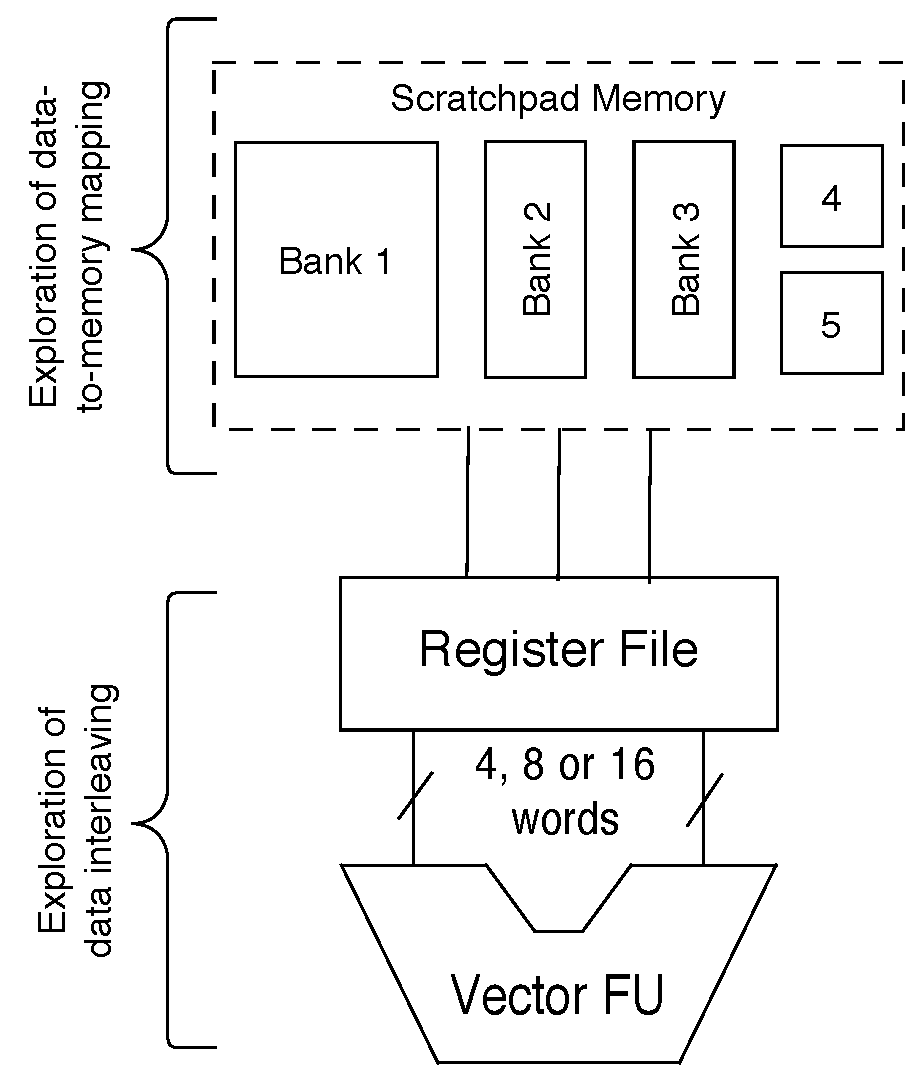
\includegraphics[scale = 0.6]{Images/Architecture.eps} 
	\caption{Exploration options and system knobs depending on a general platform architecture}
	\label{fig:arch}
\end{figure}

\subsection{Memory Models}

The dynamic memory organisation is constructed using commercially available SRAM memory models (MM).
For those models delay and energy numbers are derived from a commercial memory compiler.
In addition, experimental standard cell-based memories (SCMEM) \cite{Mei11}  are  considered for smaller memories due to their energy and area efficiency for reasonably small storage capacities, as argued in \cite{Mei10}. 
The standard cell-based memories are synthesized using Cadence RTL compiler for TSMC 40nm standard library. 
Afterwords, power simulations on the synthesized design are carried out using Synopsys PrimeTime, in order to obtain energy numbers.
Both MMs and SCMEMs can operate under a wide range of supply voltages, thus support different operating modes that provide an important exploration space.
\begin{itemize}
\item Active mode: The normal operation mode, in which the memory can be accessed at the maximum supported speed. The supply voltage is 1.1V. 
The dynamic and leakage power are higher compared to the other modes.
Only on active mode the data are accessible without time penalties, in contrast to light and deep sleep modes.
In this work all the memory accesses are performed in active mode. 
\item Light sleep mode: The supply voltage in this mode is lower than active with values around 0.7V. 
The access time of the memory is significantly higher than the access time in active mode. 
Switching to active mode can be performed with a negligible energy penalty and a small time penalty of a few clock cycles (less than 10). 
Data is retained.  
\item Deep sleep mode: The supply voltage is set to the lowest possible value that can be used without loss of data. 
This voltage threshold is expected to be lower for SCMEMs than MM models and can be as low as 0.3V. 
The number of clock cycles needed for switching to active mode is higher compared to sleep mode, typically in the range of 20 to 50 clock cycles depending on the clock speed. 
Consequently, the speed of the PE and the real-time constrains of the applications has to be taken into consideration when choosing light or deep sleep mode at a specific time.  
\item Shut down mode: Power-gating techniques are used to achieve near zero leakage power. 
Stored data is lost. 
The switch to active mode requires substantially more energy and time. 
However, switching unused memories to this mode, providing that their data are not needed in the future, results in substantial energy savings.
\end{itemize}  

The necessary energy and power information is available for the memory models and relative values for a subset of them is presented in Table \ref{tab:models}. 
It is clearly shown that the choice of memory units has an important impact on the energy consumption.

\begin{table}
\tbl{Relative dynamic energy for a range of memories with varying capacity and type\label{tab:models}}{
	\begin{tabular}{|c|c|c|c|c|c|}
		\hline
		\multirow{2}{*}{\textbf{Type}} & \textbf{Lines x} & \multicolumn{2}{c|}{\textbf{Dynamic Energy [J]}} & \multicolumn{2}{c|}{Switching to Active from} \\ \cline{3-4}
		& \textbf{wordlength} & Read & Write  & Deep[uJ] & Light[uJ]\\ 
		\hline 
		MM & 32 x 8 &  $ 4.18 \times 10^{-8} $ &  $ 3.24 \times 10^{-8} $ & 0.223 &  0.031 \\ 
		\hline
		MM & 32 x 16 & $  6.79 \times 10^{-8} $ &  $ 5.89 \times 10^{-8} $ & 0.223 &  0.031\\ 
		\hline
		MM & 32 x 128 & $  4.33 \times 10^{-7} $ &  $ 4.31 \times 10^{-7} $ & 1.42 & 0.168\\ 
		\hline
		MM & 256 x 128 & $  4.48 \times 10^{-7} $ &  $ 4.60 \times 10^{-7} $ & 1.70 &  0.171\\ 
		\hline
		MM & 1024 x 128 & $  5.11 \times 10^{-7} $ &  $ 5.75 \times 10^{-7} $ & 2.81 & 0.179\\ 
		\hline
		MM & 4096 x 128 & $  9.60 \times 10^{-7} $ &  $ 4.57 \times 10^{-7} $ & 9.01 & 0.457\\ 
		\hline
		SCMEM & 128 x 128 & $  2.5 \times 10^{-7} $ &  $ 0.8 \times 10^{-8} $ & 1.51 &  0.045\\ 
		\hline
		SCMEM & 1024 x 8 & $  1.7 \times 10^{-8} $ &  $ 0.6 \times 10^{-8} $ & 0.325 &  0.021\\ 
		\hline
	\end{tabular}}
\begin{tabnote}%
\Note{Source:}{\cite{filippopoulos2013exploration}}
\end{tabnote}%	
\end{table}

\subsection{Function Unit Models}

The processing of the interleaved data is performed in the part of the architecture consisting of the SIMD FU and the central vector register file, as shown in Fig.\ref{fig:arch}.
For efficient utilization of the vector FU, the register file has a wide interface (256 bit wide) with the scratchpad memory and allows testing for word length of 4, 8 and 16 elements, assuming that each array element is a 16 bit wide.  
This processor belongs to the class of coarse-grain reconfigurable array (CGRA) processors and is described in more detail in \cite{lee2003compilation}.
The HDL model of the processor is synthesized using Cadence RTL compiler \cite{cadencecompiler} and the energy numbers are extracted using Synopsys Primepower \cite{kai2003synopsys}.

For efficient utilization of the vector FU, the register file has a wide interface with two scratch-pad memories. 
Since the target architecture is a configurable processor that can be customized in various ways, the standard evaluation and execution mechanism is to run the programs on a processor simulator. 
An XML based language is used to describe the architecture, and a cycle-accurate simulator of the processor is used to simulate the generated code on the architecture. 
The energy consumption information for different type of instructions and different widths is available for the FU models.
The width of the FU corresponds to the number of pairs of array elements on which the specific instruction is performed.
Relative values for a subset of them is presented in Table \ref{tab:models2}. 
It is clearly shown that the wider FUs have a significantly higher energy consumption compared to FUs that operate on only two element.
Thus, it is important to achieve high utilization of wider FUs to achieve both performance and energy gains.

\begin{table}
\tbl{Relative dynamic energy for different FU models\label{tab:models2}}{
	\begin{tabular}{|c|c|c|}
		\hline
		\textbf{Type of FU instruction} & \textbf{Width} & \textbf{Dynamic Energy [J]} \\ 
		\hline 
		ADD  & 1 & 5.70E-08 \\ 
		\hline
		ADD  & 4 & 2.28E-07 \\ 
		\hline
		MULT  & 1 & 2.48E-07 \\ 
		\hline
	 	MULT complex  & 1 & 5.33E-07 \\ 
		\hline
		MULT  & 4 & 1.03E-06 \\ 
		\hline
		MULT complex  & 4 & 1.95E-06 \\ 
		\hline
		\end{tabular}}
\begin{tabnote}%
\Note{Note:}{Models for multiplication are different based on the type of input variables.}
\end{tabnote}%	
\end{table}

\section{System Design Exploration Work-flow}
\label{sec:methodology}

\begin{figure}
\centering
	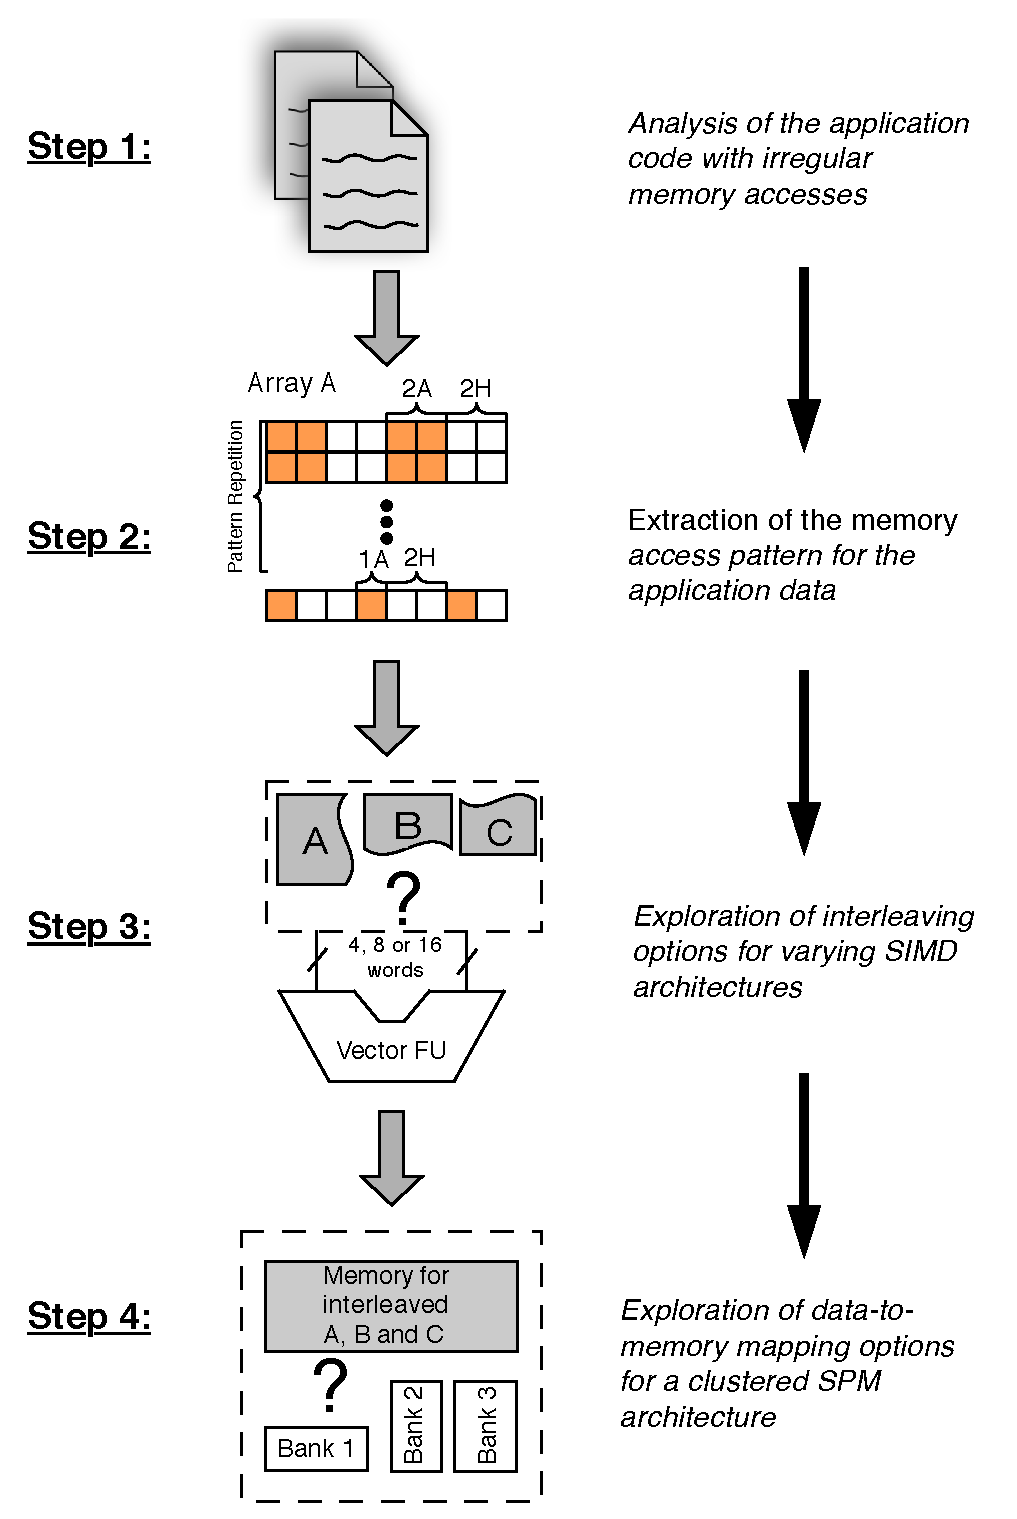
\includegraphics[scale = 0.6]{Images/workflow2.eps} 
	\caption{Methodology steps}
	\label{fig:workflow}
\end{figure}

The systematic exploration of the interleaving options and the data-to-memory mapping possibilities is necessary.
The input of work-flow is the application code and the output of the exploration is an efficient solution for the interleaving of the data and a reconfigurable system architecture based on the available models presented in Sec.\ref{sec:platform}.
The exploration space consists of the potential combinations between the different arrays and the different scratch-pad memory architectures, which combine memories of different types and sizes.

The overall work-flow of this work is presented in Fig.\ref{fig:workflow}. 
The first step of the methodology is the analysis of the application code. 
The methodology is applicable to any application.
However the applications that can benefit more from the proposed methodology are the ones with irregular access patterns.
The second step is the extraction of the access pattern for each data structure present on the application code.
The third step is the interleaving exploration, which explores all the different options for the re-arrangement of the data.
The aim of this step is the construction of compact sets of data by using defined operations between the available access patterns.
The goal is to better utilize the different width of the vector FUs. 
The result of the interleaving is a set of data with a reduced number of holes.
The forth step is the mapping of the interleaved data set to the clustered memory architecture.

\subsection{Formal Model Representation of Access Pattern }

A representation model for the access pattern is employed in order to formally present each step of the methodology.
The model presented in \cite{Ang13} is a generic model suitable for irregular iteration spaces on arrays.
The irregularities are created by the application code access statements in a conditional loop structure.

When an array element is accessed, during the code execution, is represented with an A(Access).
Otherwise, there is a hole in the access pattern represented with an H(Hole) as shown in Fig.\ref{fig:pattern}.
The sequence of accesses and holes is usually repeated periodically, because normally the loop conditions are not totally random.
Thus we can define the frequency of each access pattern.
The analysis of the application code results in the access patterns and their corresponding frequencies, which is the necessary input for the next step on the work-flow.

\begin{figure}
\centering
	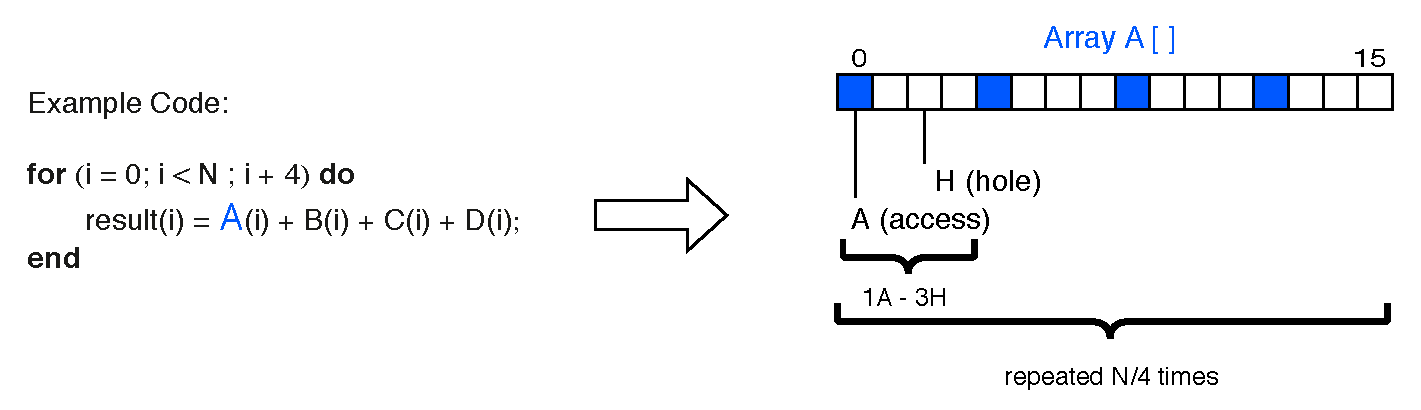
\includegraphics[scale = 0.6]{Images/AHpattern.eps} 
	\caption{Extraction of access pattern from application code}
	\label{fig:pattern}
\end{figure}

%\textit{Discussion about polyhedral and enumerative approaches}
%\textit{Analysis of A-H model based on Angeliki}
%\textit{Definition of algebra functions between access patterns}

\subsection{Data Interleaving Exploration}
Interleaving is a data layout transformation for combining the storage of multiple arrays, so that blocks of data from different arrays are stored contiguously, in order to achieve spatial locality in memory accesses.
By interleaving we are able to group the data to be accessed and thus reduce the number of memory accesses for accessing them.
The basic principles of the performed interleaving exploration are presented in \cite{sharma2013data}.

The employed model of access pattern representation is accompanied with a suitable algebra presented in \cite{kritikakou2013phd}.
The operations defined help the designer explore different interleaving options.
The goal of the process is to rearrange the data in a more efficient way that increases the number of sequential accesses.
A simple example is presented in Fig.\ref{fig:algebra}.
Arrays $A$ and $B$ are interleaved by interchangeably storing an element of each array in the new array. 
The access patterns of arrays $A$ and $B$ are combined in a new access pattern, which has two accessed elements placed consequentially.
The use of access patterns and the theory for calculating the access patterns of different combinations enables an extensive exploration of the possible data interleaving options.

The impact of the data interleaving exploration on the number of memory accesses is significant.
When the accesses are irregular and the data are organized in index order, each memory access results in a small amount of useful data due to the presence of holes.
In contrast the re-organization of the data provides a sequence of useful data without many holes between them.
Thus, a single access to the memory results in a higher number of useful elements.
The overall number of memory accesses is reduced, as each access has a higher utilization.

This idea is illustrated in Fig.\ref{fig:algebra}.
The number of memory accesses for each case can be calculated by assuming that each memory access loads four array elements, i.e. the word length for the memory and bus architecture is four elements.
Each time an element from the array $A$ or $B$ is needed, the memory access returns four elements, from which one is the useful and the other three are not used by the running code.
On the case of the interleaved array, each memory access returns four elements, from which two are useful and two redundant.
Thus, the number of overall memory access in the second case is reduced in half compared to the first case.

\begin{figure}
\centering
	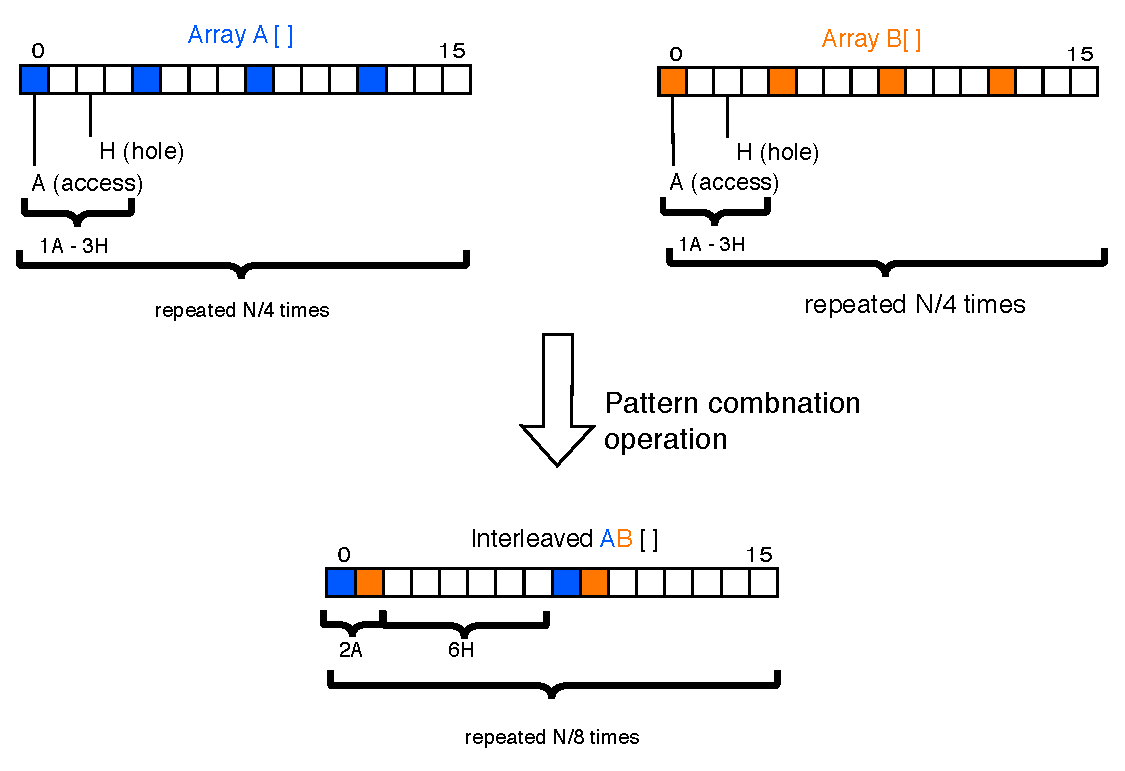
\includegraphics[scale = 0.6]{Images/Algebra.eps} 
	\caption{Example of combination between two arrays and their access patterns}
	\label{fig:algebra}
\end{figure}
%\textit{Algorithm for exploring data interleaving}

\subsection{Data-to-Memory Mapping Exploration}

Given the input from the previous step, we explore the mapping of the interleaved data to the memory architecture.
A clustered memory organisation with up to five memory banks of varying sizes is explored. 
The limitation in the number of memory banks is necessary in order to keep the interconnection cost between the processing element (PE) and the memories constant through exploration of different architectures. 
The decision to use memory banks with varying sizes on the clustered memory organization increases the reconfiguration options and consequently the potential energy gains. 
In general, smaller memories are more energy efficient compared to larger memories banks. 
However, in some cases large memory banks are needed in order to fit the application data without the need for too many small memories causing complex interconnects. 
The goal is to use the most energy efficient banks to store the interleaved data.

The exploration space consists of different sizes and types of memory banks.
The goal is to make the optimal decision regarding the mapping of the data to the different memory banks.
The parts of the interleaved data that consist mostly of useful elements are mapped into memory banks with low energy per access.
The parts of the interleaved data that consist of access holes and rarely accessed elements are optimally mapped into memory banks with energy efficient retention states.
In both cases the size of  the memory banks should be adequate to fit the stored data but at the same time as small size as possible to avoid area and energy penalties.

\subsection{One way constraint propagation}

The interleaving decisions influence the data-to-memory mapping decisions and vice versa.
For example, the decision to interleave two arrays \textit{A and B} have an impact on the freedom of mapping the interleaved array $A\vert B$ on the memory banks, because of its different size and structure.
The data-to-memory mapping decisions affect the interleaving decisions on a similar way.
Assuming that the mapping is performed on the initial data the interleaving options are reduced.
For example, the decision to map two arrays on different memory banks removes the option to interleave them later.
Optimizing both the interleaving and the memory mapping at the same time results in a large and inefficient loop of constrain propagations between the two exploration phases.
 
We choose to perform the interleaving exploration step first and then propagate the most efficient interleaving options to the data-to-memory mapping step.
The code and data transformations should be performed earlier to avoid omitting possible solutions as justified in \cite{dtse}.
Thus, the interleaving decisions are propagated as constraints on the mapping exploration phase. 
The constrains consist of the arrays that are interleaving, the new access pattern and the width of SIMD architecture for which the specific interleaving solution is optimal.
The mapping step is performed based on the constrains and the suitable solutions for mapping the interleaved data to memory are given.

\section{Applications}
\label{sec:applications}

The applications that benefit most from the proposed methodology are characterised by having irregular access patterns with holes.
The multimedia domain offers some suitable candidates for the presented methodology.
An overview of the tested benchmark applications is presented below:

\begin{enumerate}
\item Motivational example is the very simple example presented in Sec.~\ref{sec:motivational}. 
It uses four arrays that all have the same irregular access pattern, namely 1A-3H.
One element from each array is used to calculate an intermediate result on every loop iteration.
The interleaving is easy because the four arrays has the same pattern.
Further interleaving within the array can result into even longer sequences of useful elements.
The access pattern is repeated for every four elements (1A-3H), so the scaling for the different word lengths (4, 8 and 16) is expected to be good. 
\item Successive Over Relaxation (SOR) is a method for evaluating partial differential equations or solving linear system of equations.
The SOR benchmark has a more irregular access pattern.
The interleaving exploration provides sequences of three or six sequential useful elements.
Thus, the utilization on the SIMD architecture is expected to be lower.
\item FFT benchmark has an irregular pattern during the access of the pilot matrices. 
The interleaving exploration for FFT is presented in \cite{sharma2013data}.
The number of matrices is higher and more interleaving options are present.
However, the interleaving cannot provide an acceptable solution for 16 sequential useful elements.
\item Motion estimation benchmark is a dynamic algorithm that results in different access patterns based on the identification of the moving objects. 
The static parts are not accessed resulting in holes in the accesses and the interleaving aims to minimize those parts.
The interleaving exploration provides alternatives for all the  tested word lengths. 
\end{enumerate}

\section{Results}
\label{sec:results}

%\begin{table}%
%\tbl{Normalized energy consumption\label{tab:results}}{
%\begin{tabular}{c c}
%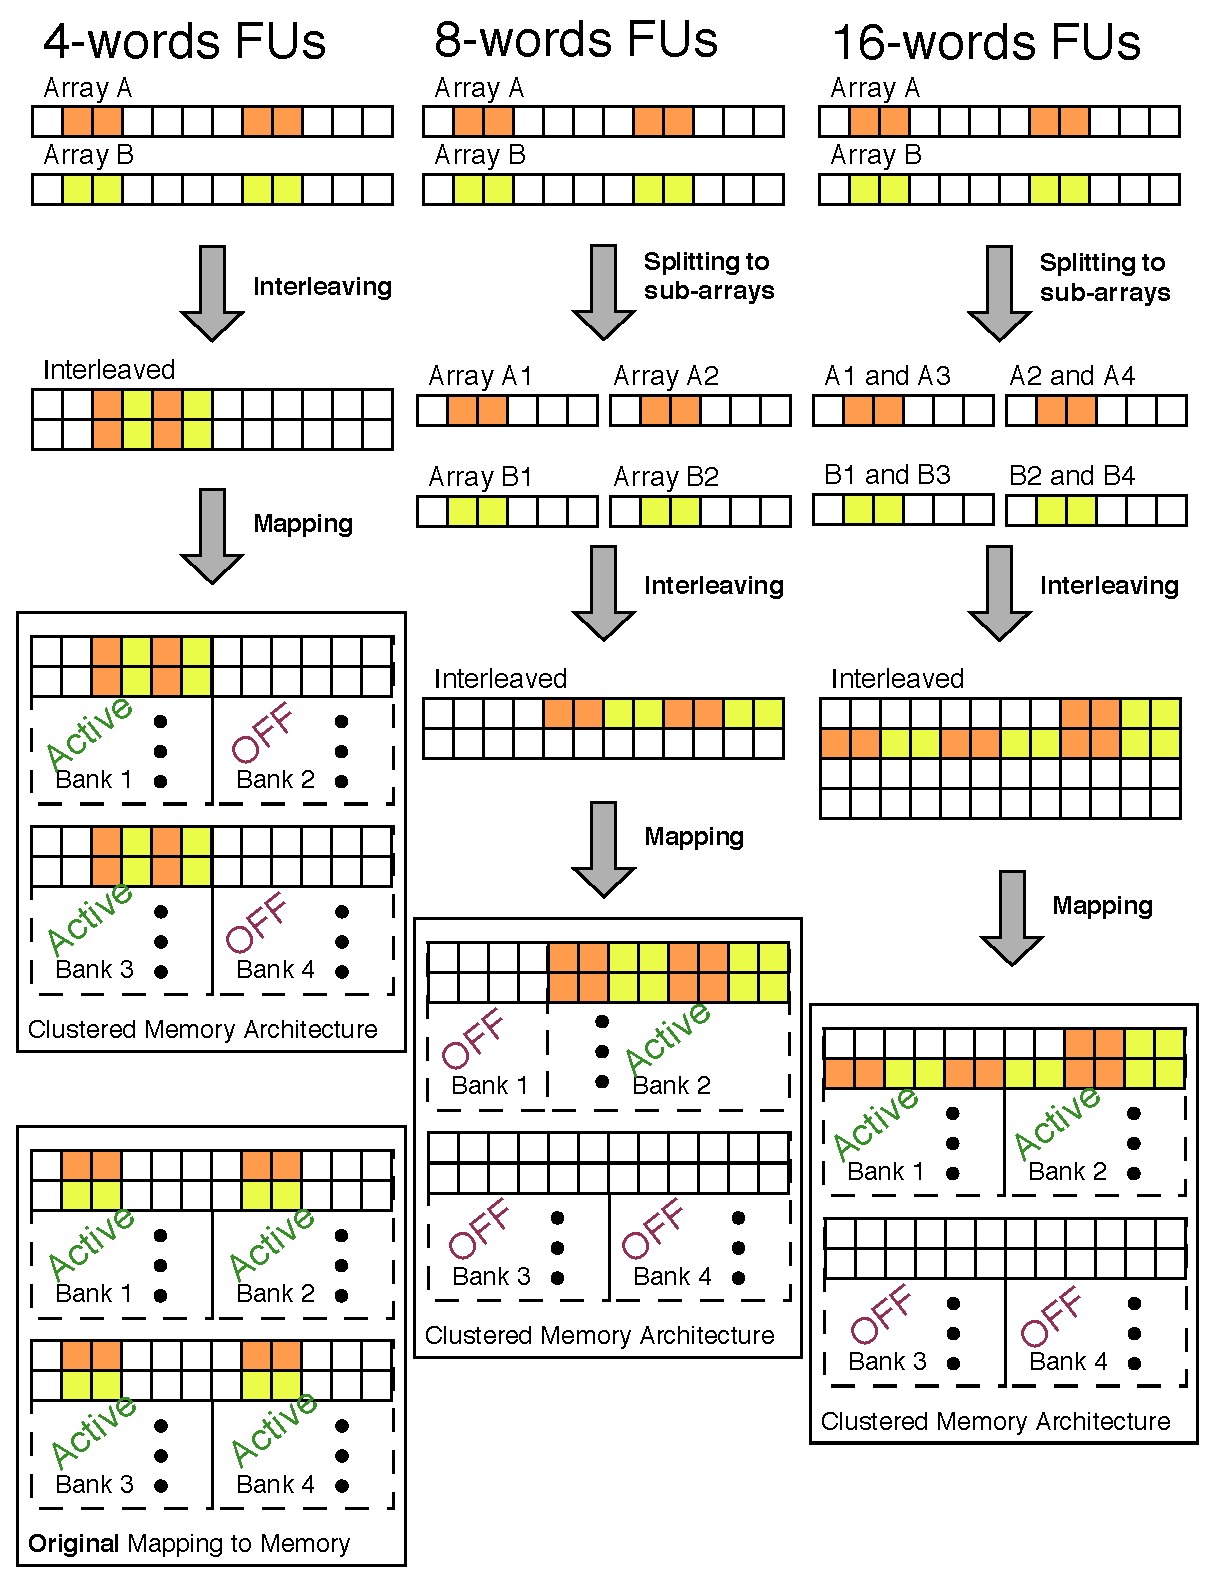
\includegraphics[width=0.45\linewidth]{Images/Example.eps} & 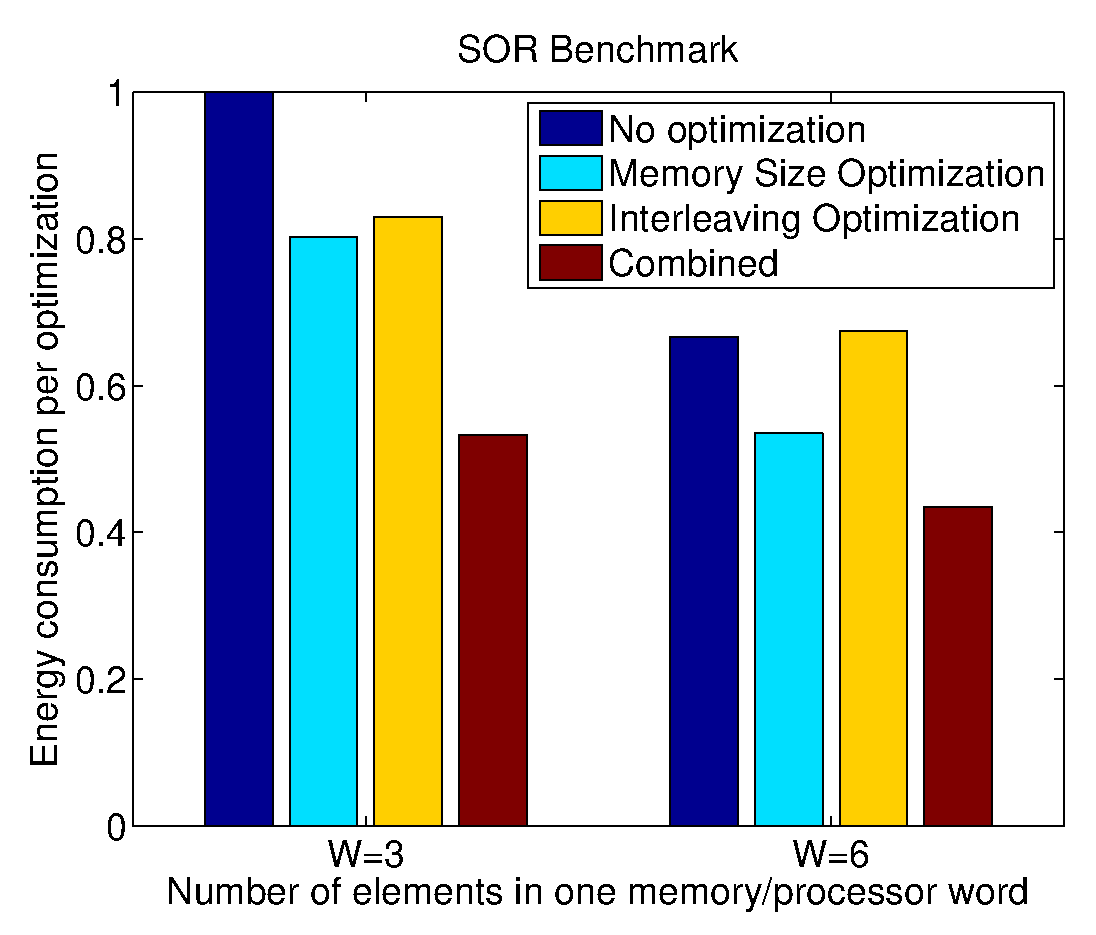
\includegraphics[width=0.45\linewidth]{Images/sor.eps} \\
%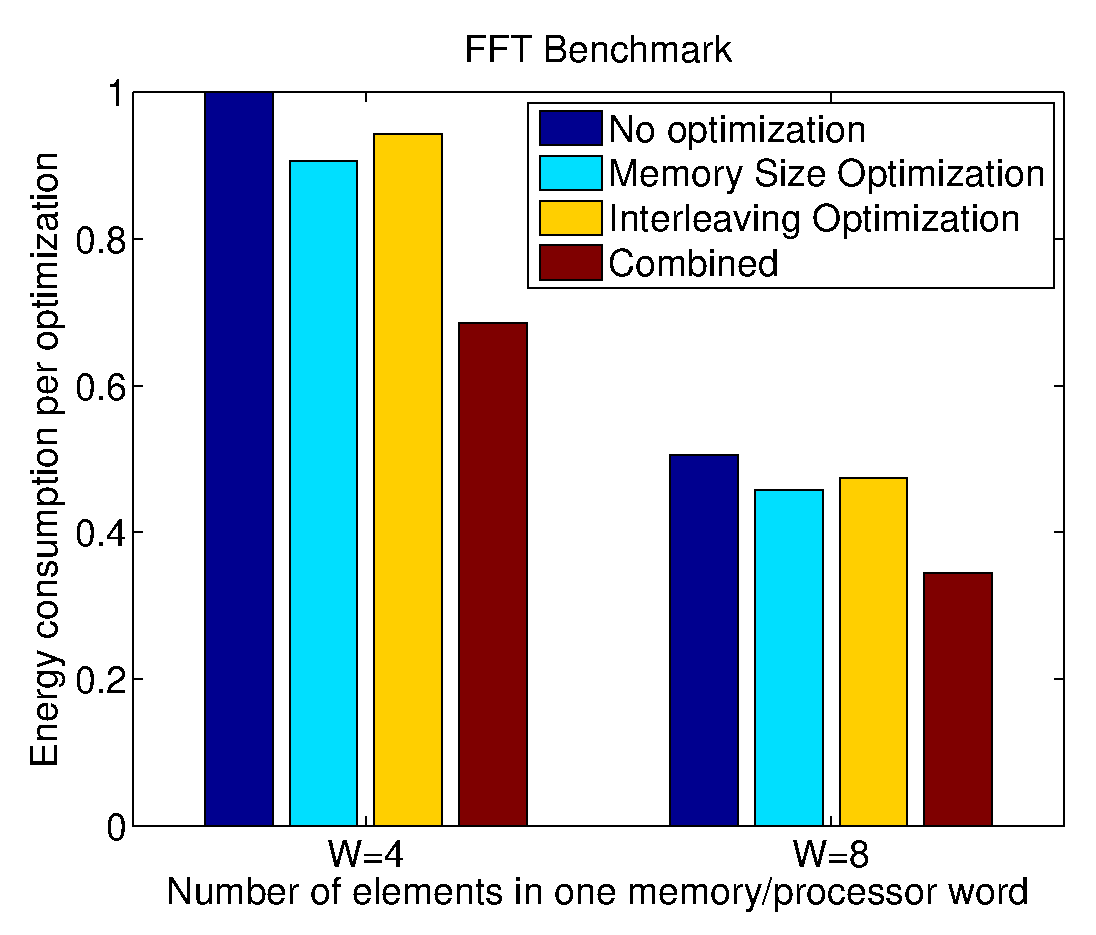
\includegraphics[width=0.45\linewidth]{Images/fft.eps} & 
%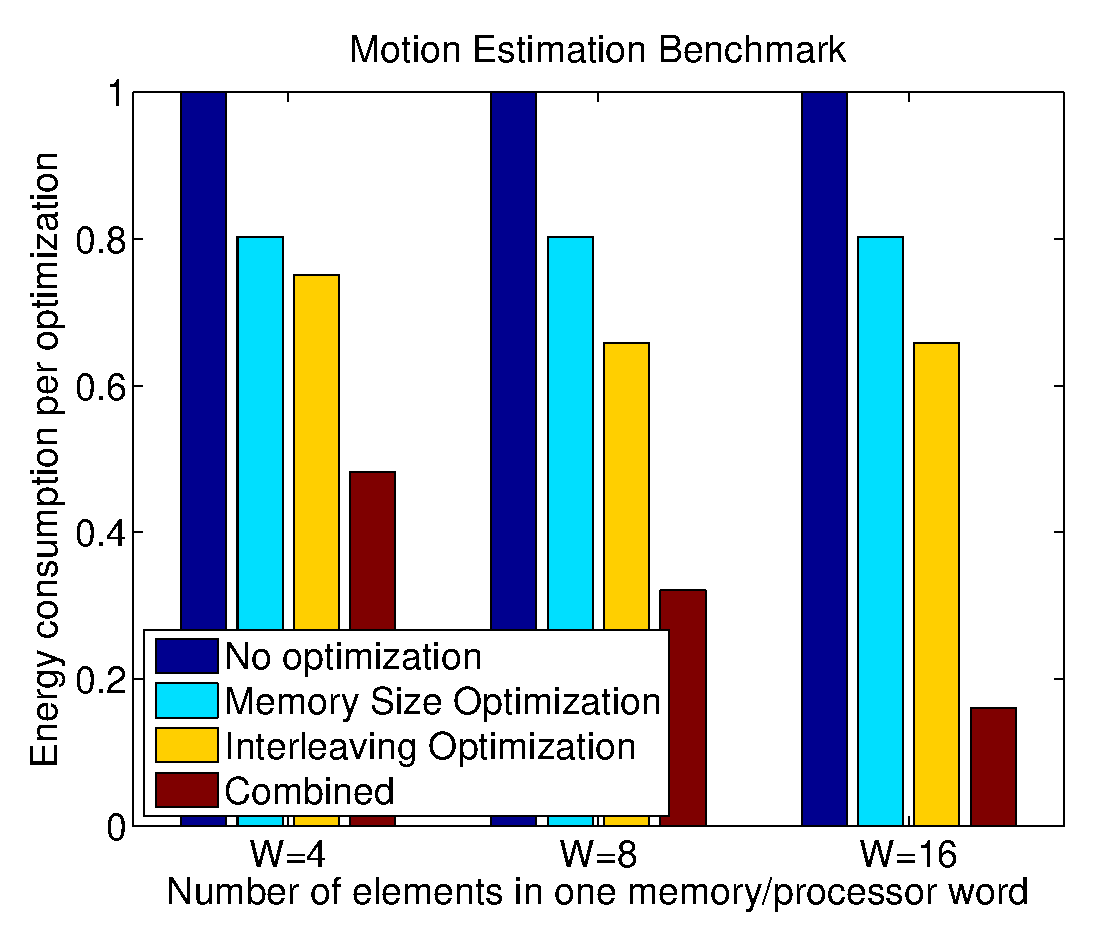
\includegraphics[width=0.45\linewidth]{Images/mest.eps} 
%\end{tabular}}
%\end{table}

The design exploration is applied to the chosen application benchmarks and energy numbers are derived based on the described target platform.
The energy numbers are calculated both for the memory and the SIMD architecture presented in Sec.\ref{sec:platform}.
Four approaches are explored and the corresponding energy consumption for each of them is calculated.

\begin{itemize}
\item \textit{No optimization.} 
In this case there is no interleaving exploration and the memory architecture consists of a large memory bank. All the data are mapped on the memory bank without any optimization. 
\item \textit{Memory Size Optimization.} 
In this case there is no interleaving exploration and the memory architecture consists of five memory banks.
The optimal size for the memory banks and the optimal mapping of the non-interleaved data on them is explored. 
The number of memory accesses is the same as in the previous approach.
However, the data is mapped on an efficient clustered memory architecture.
\item \textit{Interleaving optimization.} 
In this case the  interleaving exploration step is performed and the memory architecture consists of one large memory bank.
The optimal interleaving decision is found and applied to the data, so the locality of useful data is increased.
However, all the data are mapped on one large memory bank.
The number of accesses is significantly reduced by the interleaving step, but the energy per access is kept high due to lack of data mapping to an efficient clustered architecture.
\item \textit{Integrated co-exploration.} 
In this case the co-exploration of both the interleaving and the data-to-memory mapping optimizations is performed.
Both he number of memory accesses and the energy per access are reduced.
\end{itemize}

\subsection{Motivational Example}

\begin{figure}
\centering
	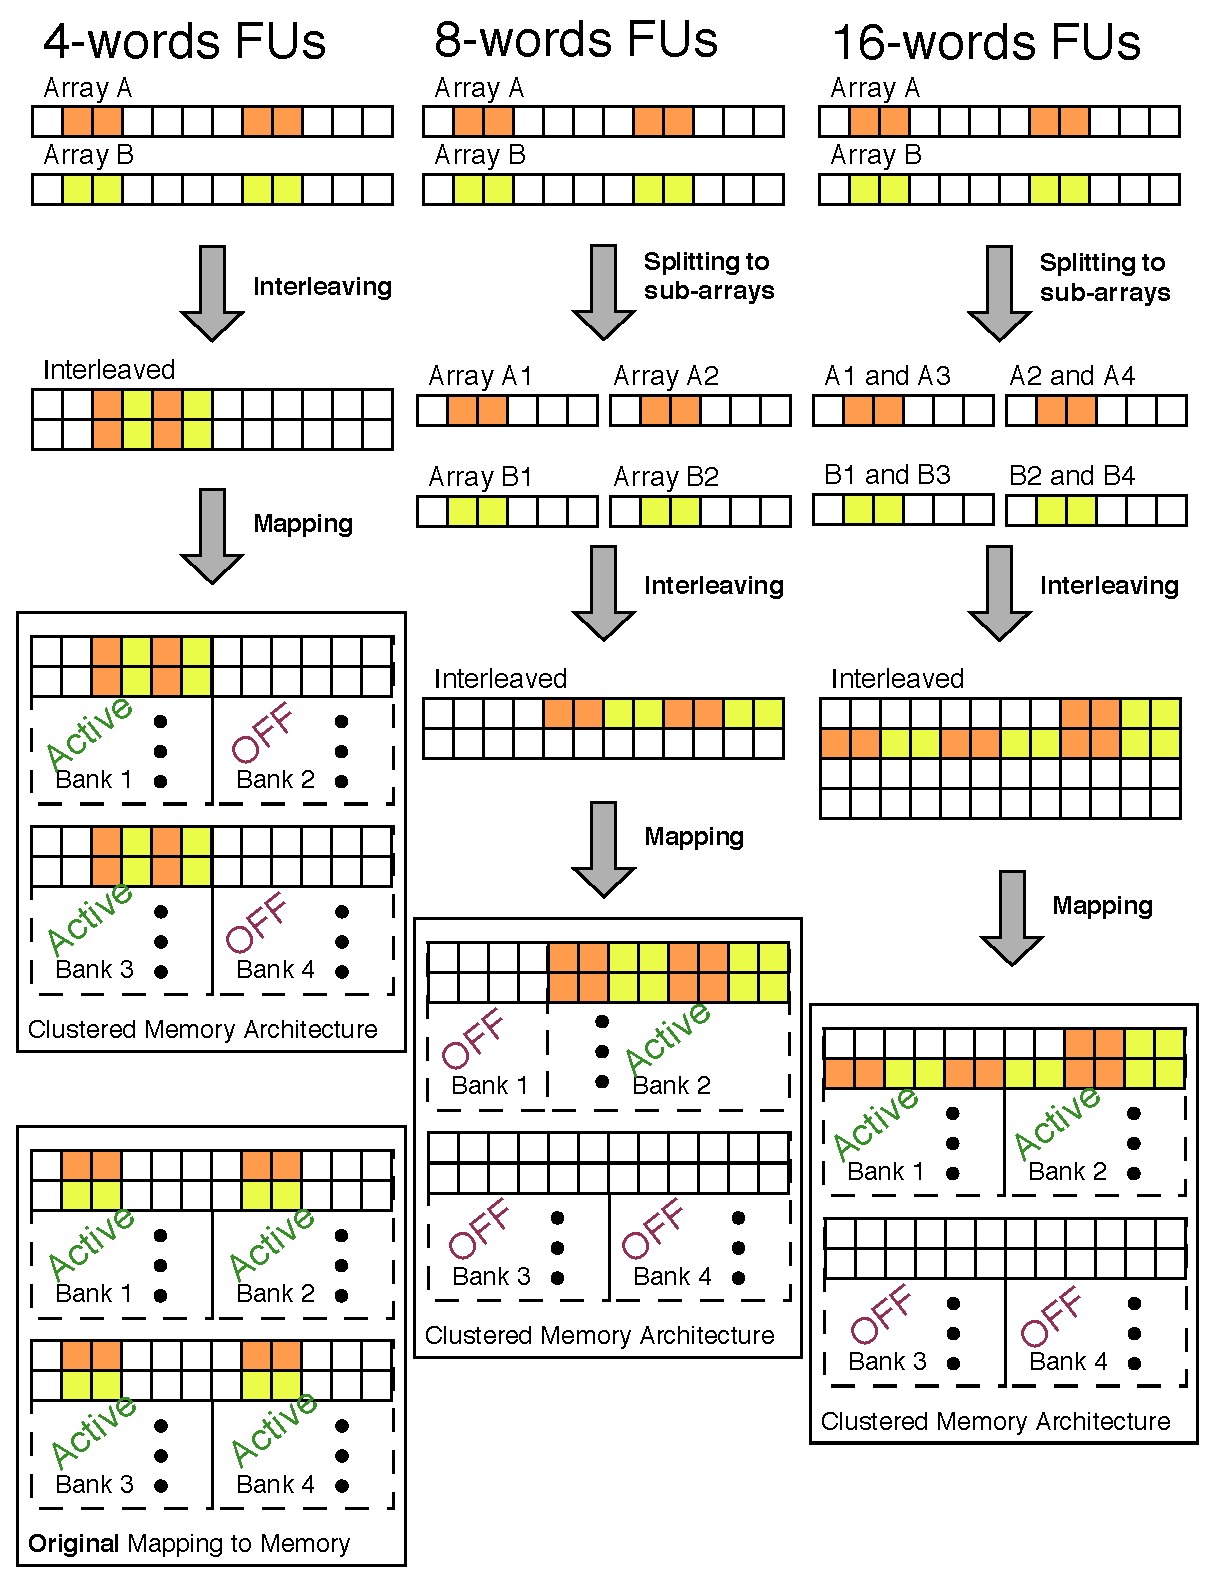
\includegraphics[scale = 0.5]{Images/Example.eps} 
	\caption{Motivational Example}
	\label{fig:example}
\end{figure}

The normalized energy consumption for the motivational example is presented in Fig.\ref{fig:example}.
The four different approaches are normalized using the conventional case without any optimization.
Energy results for this benchmark are presented for a word length of 4, 8 and 16 elements, which means that every memory access loads/stores 4,8 or 16 elements. 
The interleaving exploration proposes three different solutions for an SIMD architecture width of 4, 8 and 16 elements respectively.
The data access patterns of the three interleaving decisions are propagated as a set of constrains to the mapping step.
The mapping step explores all the different data-to-memory mapping options and proposes the most energy efficient memory organization for each of the three interleaved data solutions.

The application code is perfectly suitable for interleaving as discussed in Sec.\ref{sec:motivational}.
Thus the interleaving exploration has a greater impact that the memory size optimization.
However, the integrated approach optimizes the energy consumption even further.
The application is suitable for higher word lengths and there are important gains while moving from 4 to 8 and 16.
The increase in the architecture width result in significant gains even without any optimization.
The gains are approximately 50 and 70\% for a width of 8 and 16 compared to a width of 4.
This is explained by the fact that the accessed array elements are close enough even without data transformations and the existence of holes in the access pattern. 
By fetching 8 and 16 elements from the memory, the number of useful elements is two and four times more.
Studying the motivational example in Fig.\ref{fig:example}(a) for a width of 16, each fetching results in 4 lines with one coloured element each.

The interleaving optimization results in greater improvements compared to the memory optimization.
This is explained by the nature of the application that offers good interleaving options for larger words, i.e. higher values of width.
The memory optimization is around 20\% lower than the monolithic approach for any width.
The interleaving optimization results in more than 70\% lower energy for a width of 4 and more than 80\% for a width of 8 and 16.
The interleaving of the arrays provides perfectly compact sets of data as shown in Fig.\ref{fig:example} and the interleaving cannot improve more for higher values of width.
The great impact of the combined approach is better illustrated for a width of 16. 
In this case the two optimizations alone report an energy gain around 20\% and 35\% compared to the non optimized case for width of 16.
The combined approach results in an energy gain of 84\% on the same case.

\subsection{SOR Benchmark}

\begin{figure}
\centering
	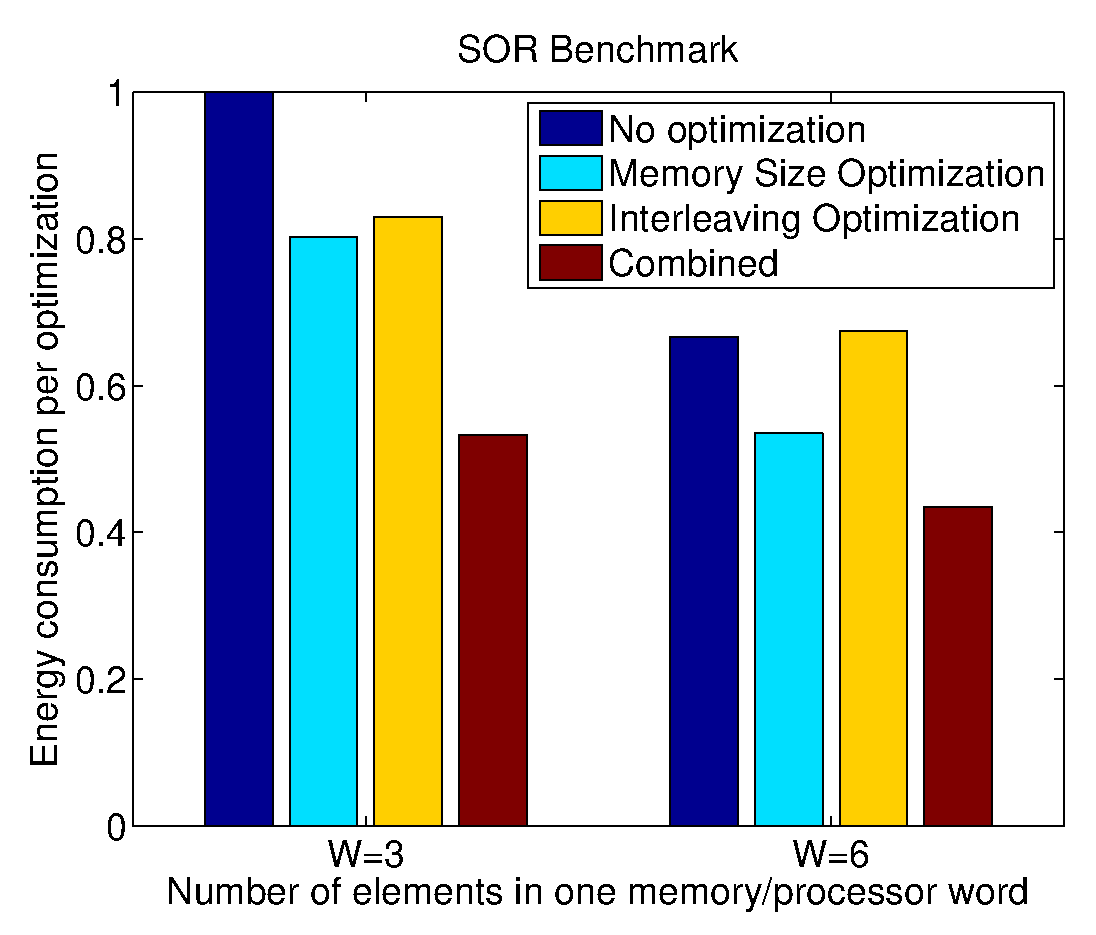
\includegraphics[scale = 0.5]{Images/sor.eps} 
	\caption{SOR Benchmark}
	\label{fig:sor}
\end{figure}

The normalized energy consumption for the SOR benchmark is presented in Fig.\ref{fig:sor}.
The four different approaches are normalized using the conventional case without any optimization.
Energy results for this benchmark are presented for a word length of 3 and 6, which means that every memory access loads/stores 4 or 8 elements, because the architecture supports word lengths in the power of 2.
This limitation is due to the nature of the application code that adds elements from 3 arrays to 3 constant elements of another array. 
The interleaving exploration on the application code concludes that it is only possible to make sequential sets of 3 and 6 elements by interleaving the arrays of the application.
Thus the interleaving exploration alone has a small impact on the reduction of energy consumption for word length of 3 elements.
The results are even worst for a word length of 6 elements, because the interleaved data have greater size and the conventional mapping of them to the memory is poor.
The memory size optimization provides more important reduction.
The integrated approach exploit on a better way the few interleaving options by providing a better mapping of the interleaved data to the memory architecture.

\subsection{FFT Benchmark}

\begin{figure}
\centering
	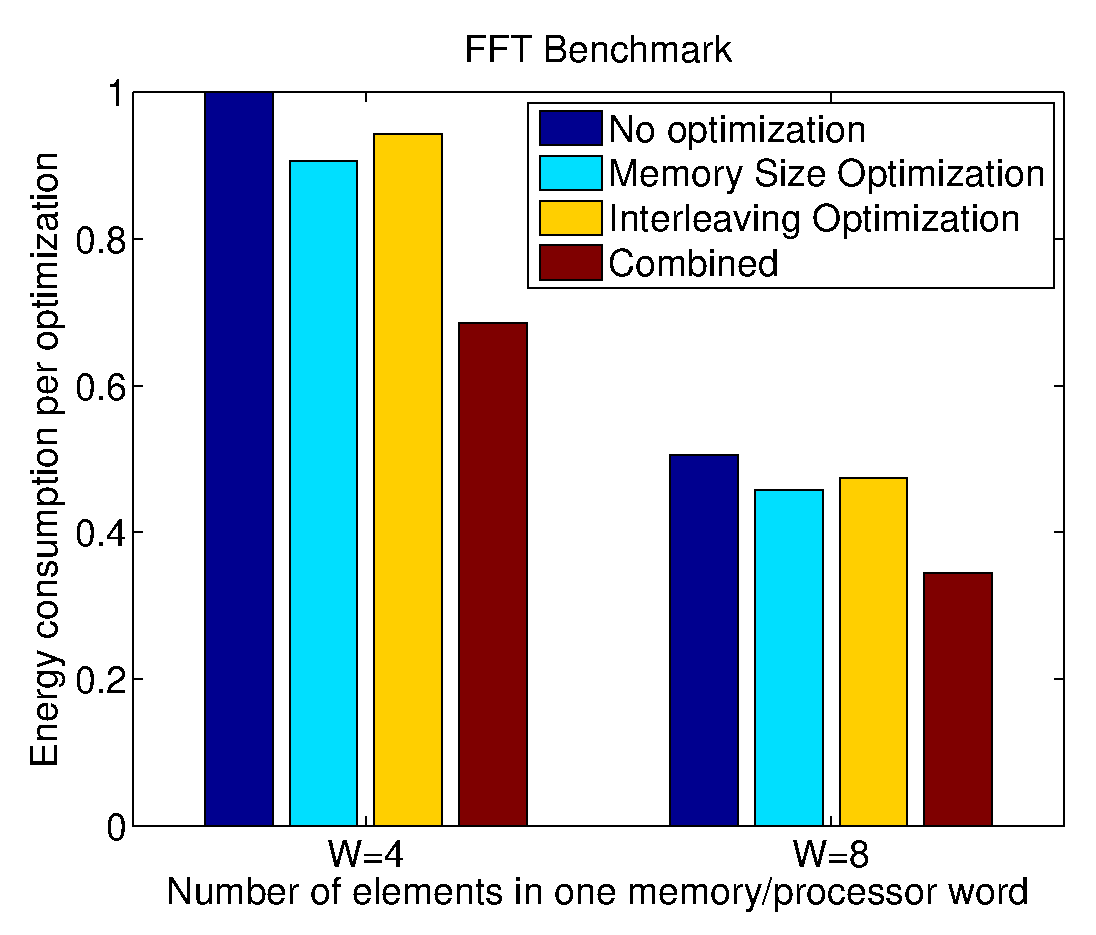
\includegraphics[scale = 0.5]{Images/fft.eps} 
	\caption{FFT Benchmark}
	\label{fig:fft}
\end{figure}

The normalized energy consumption for the FFT benchmark is presented in Fig.\ref{fig:fft}.
The four different approaches are normalized using the conventional case without any optimization.
Energy results for this benchmark are presented for a word length of 4 and 8 elements, which are the two viable options provided by the interleaving exploration.
Again, the integrated approach results in the lower energy consumption.
The energy gains for a word length of 8 are significantly high, because blocks of 8 words can be constructed by interleaving of application's arrays.

\subsection{Motion Estimation Benchmark}

\begin{figure}
\centering
	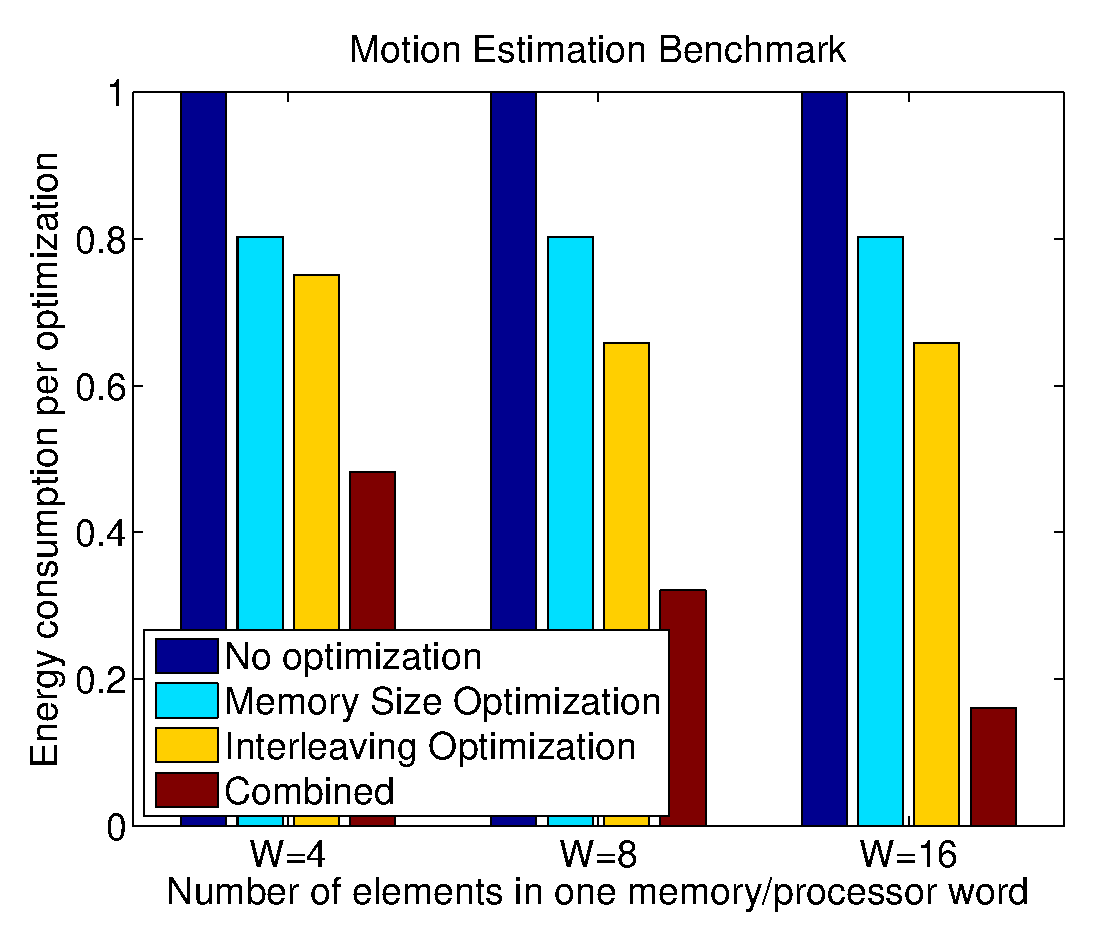
\includegraphics[scale = 0.5]{Images/mest.eps} 
	\caption{Motion Estimation Benchmark}
	\label{fig:mest}
\end{figure}

The normalized energy consumption for the motion estimation benchmark is presented in Fig.\ref{fig:mest}.
The four different approaches are normalized using the conventional case without any optimization.
Energy results for this benchmark are presented for a word length of 4, 8 and 16 elements.
The application code provides good possibilities for interleaving and consequentially the interleaving exploration has a greater impact that the memory size optimization.
However, the integrated approach optimizes the energy consumption even further.
In this case the energy gains for increasing size of word length are minimal.
This is explained by the nature of the application...

\section{Conclusion}
\label{sec:conclusion}

The scope of this work is to presents a methodology for efficient exploration of data interleaving and data-to-memory mapping options for SIMD (Single Instruction Multiple Data) platform architectures.
Detailed energy models are presented for the studied architecture.
The methodology focuses on reducing the overall energy consumption by reducing the number of memory accesses and the energy per access.
The number of memory accesses is reduced by interleaving the application data to construct compact sets of sequential data.
The energy per memory access is reduced by employing a reconfigurable scratch-pad memory architecture with multiple banks that can operate independently.
A systematic way is presented in order to explore the different options that lead to the interleaving and data-to-memory mapping decisions.
A wide range of applications is studied that allow us to draw conclusions about different kinds of dynamic behaviour and their effect on the energy gains achieved using the methodology. 
The presented methodology is tested using a number of benchmark applications with irregularities on their access scheme.
The improvement on the energy consumption after efficient interleaving and mapping of data is approximately between 40\% and 80\% for the complete system and the studied benchmarks.

% Bibliography
\bibliographystyle{ACM-Reference-Format-Journals}
\bibliography{reference}

\end{document}